\documentclass[11pt]{article} 
\usepackage{algorithm}
\usepackage{algorithmic}
%\usepackage{algpseudocode}
\usepackage[utf8]{inputenc} 
\usepackage[left=1.5cm,top= 1.5cm,right= 1.5cm,bottom=1.5cm]{geometry} 
\usepackage{amsmath,amssymb,amsfonts,latexsym} %Soporte para símbolos y font matemáticos
\usepackage{graphicx}			      %Soporte para gráficos.
\usepackage{float}
%\usepackage{dsfont}
\usepackage{enumerate}
\usepackage{amsthm}
% \usepackage[options]{algorithm2e}
\DeclareGraphicsExtensions{.pdf,.png,.jpg}
\DeclareGraphicsRule{.wmf}{bmp}{}{}

\begin{document}
\begin{enumerate}
 \item 
 
 
 
 
 
 
 
 
 \item ¿Para qué valores de $n$ el algoritmo de inserción directa es mejor 
 que mezcla directa? 
 \[
  Inserci\acute{o}n \ directa : \ \ \ 8(n^2)\]
  \[
  Mezcla\ directa: \ \ \ 64n*log(n)
 \]
 \textbf{Respuesta en forma analítica:} \\ 
  Para saber que algoritmo es mejor que otro nos basamos en diferentes 
  métricas en las que podemos cuantificar cual es la cantidad
  de recursos que son requeridos para resolver la tarea. Estos 
  recursos principalmente se dividen en dos, el tiempo de ejecución del
  algoritmo y la cantidad de memoria que el algoritmo requiere.\\
  Implícitamente podemos medir el tiempo de ejecución si conocemos 
  cuantas instrucciones ejecutará el algoritmo, debido  a que 
  cada una de nuestras computadoras puede ejecutar un número determinado
  de instrucciones por segundo, es por ello que para conocer el número
  de segundos que tomará un algoritmo en finalizar queda determinado 
  por:
  \[
   Tiempo (s) =\frac{\#\ instrucciones}{\#\ instrucciones\ por\ segundo\ que\ la\ computadora\ ejecuta}\ \ \ \left( \frac{instrucciones}{instrucciones/s} \right) 
  \]
   Por esa razón, para saber que algoritmo es mejor que otro 
  basta con fijarse en el número de instrucciones que cada
  uno de ellos requieren, asumiendo que la misma computadora ejecutara 
  los algoritmos.Es importante notar que   el número de instrucciones 
  es una función que depende de los datos de entrada que se le dan al 
  algoritmo. \\
  Por lo ya descrito, para conocer cuándo el algoritmo de 
  inserción directa es mejor que el algoritmo de mezcla directa se hace una análisis sobre 
  la entrada comparando la cantidad de instrucciones que cada
  uno de estos requiere.\\
  
  Con el objetivo de discernir para que valores de $n$ el número 
  de instrucciones del algoritmo de inserción directa es menor
  que el algoritmo de mezcla directa, si definimos $I$ como la función que calcula
  el número de instrucciones por cada algoritmo basta con resolver la siguiente desigualdad:
  \[
   I(Inserci\acute{o}n\ directa) \leq I( Mezcla \  directa)
  \]
  Es decir:
  \[
   8*n^2 \leq 64n*log(n)
  \]
  $\Longleftrightarrow$
  \[
   n \leq 8*log(n)
  \]
  Trabajando solo con la igualdad encontraremos el valor de $n$ en el que 
  se deja de cumplir la desigualdad estricta. es decir 
  \[
   n - 8*log(n) = 0
  \]
  Dicho algoritmo en realidad está en base 2, debido a que el análisis
  de complejidad de merge sort depende de un árbol binario completo
  es por esa razón que la altura queda representada por $log_2(n)$.
  Si graficamos esta igualdad obtenemos:
   \begin{figure}[H]
    \centering
    %trim left bottom right top
  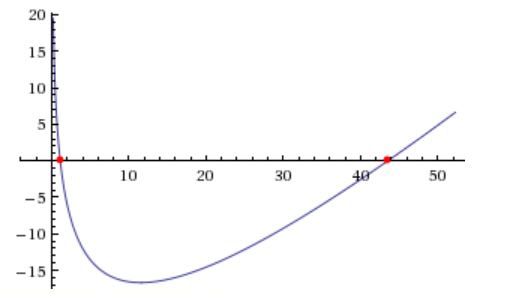
\includegraphics[trim=0cm 0cm 0cm 0cm, width=10cm]{ejercicio2_1.png} 
  \caption{Gráfica $y= n-8*log_2(n)$}
  \end{figure}
  
 
   Por lo que, la solución a la igualdad es cuando $n =1.0\overline{999}$ y $n=43$,
   con lo que concluimos que si $2 \leq n \leq 43$, entonces el
   algoritmo de inserción directa es más mejor que el algoritmo de mezcla.
   

  
  
  


  
  
  

  
 
  
  
  
 

\end{enumerate}
\end{document}
